\chapter{Introduction}
\label{chap:chap0}

While the term \emph{robotics} was first coined by Isaac Asimov some
seventy years ago, and while the first industrial robots were
developped in the 1950's, the description of automaton mechanisms can
be dated back to the tenth century B.C., which is a proof of Man's
long-time fascination with robots. The first robots had limited
capabilities, mainly focused on moving some of their limbs in order to
\emph{act} on their environment or simply to entertain. Starting from
the middle of the twentieth century, technological advances in
electronics allowed the creation of sensors which allowed robots to
\emph{perceive} their surrondings (including their own body), i.e. to
build a useful representation of them. Finally, thanks to
breakthroughs in the fields of Computer Science and Mathematics, the
means to \emph{decide} how to act based on perception were given to
robots (and roboticists too!). This decision process is known as
\emph{planning}.

\section{Anthropomorphic Systems in Robotics}

Anthropomorphic systems can be described as systems which are made to
look like humans with respect to their mechanic structure and their
abilities. In robotics, they usually have similar perception systems,
such as visual sensors in the head, tactile and inertial sensors. They
also usually have two arms and more importantly two legs, which sets
them apart from wheeled robots. These properties are such that it is
far more complex to implement a perception-planning-action on
anthropomorphic systems (or humanoid robots).

So why do we bother desigining and studying anthropomorphic systems?
Simply because it is fun! As the reader may still be sceptical with
respect to this argument, there are luckily many applications for
humanoids robotics. First of all, as humanoid robots are made to look
like humans, they have similar abilities that can allow them to walk,
run, jump, climb, write, carve, manipulate, etc. There are of course
highly specialized robots that can achieve each one of those tasks,
but very few exhibit such a high versatility. Also, we are witnessing
a shift from industrial robotics to personal robotics. Humanoid robots
can have access to the same environments as humans, and they are mode
to look like them and be easily accepted: they can therefore be used
as companions, assistants, guides, teachers, etc in various
situations.

From a research point of view, anthropomorphic systems are very
interesting subjects as they give researchers the means to devise new
algorithms to control them and make them walk and manipulate objects
without loosing their balance, allowing the generation of human-like
motions. Conversely, humanoid robots are the perfect tool for
neuroscientists to understand human motion and perception, as well as
the invariants behind them; indeed humanoid robots allow the
decomposition of complex problems into simpler ones. They also tend to
be more cooperative than humans or monkeys when it comes to accomplish
tedious and repetitive tasks during experiments.

\begin{figure}
  \centering
      {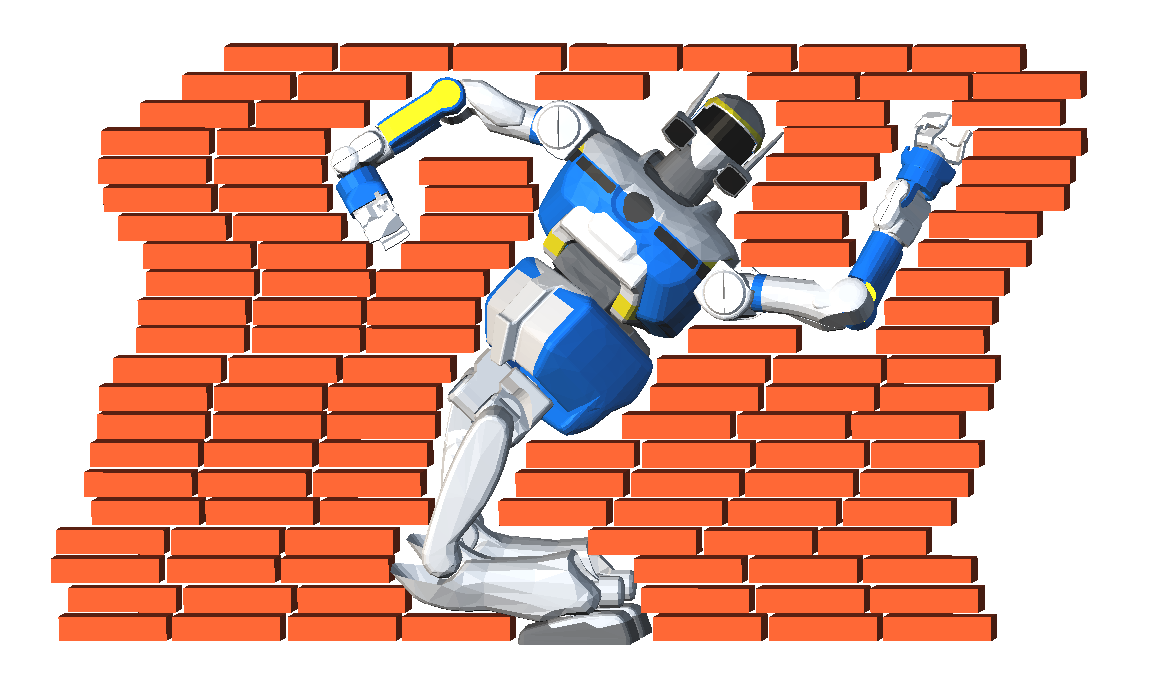
\includegraphics[width = 0.7\linewidth]
        {src/chap0-introduction/hrp2-brick-wall.png}}
      \caption{The human-like mechanical structure of humanoid robots
        allow them to accomplish complex tasks, such as avoiding
        obstacles in constrained environments.}
      \label{fig:chap0-hrp2-brick-wall}
\end{figure}

In this thesis, we focus on developping new algorithmic tools for
\emph{planning optimal motions for anthropomorphic systems}, and
applying on humanoid robots.

\section{Problem Statement}

The problem of motion planning for anthropomorhpic systems can be
defined as the following: given a starting configuration, say a
position, we would like an anthropomorphic system, say a humanoid
robot or a digital actor, to reach a goal configuration if it is
possible. Obviously such a system cannot move instantaneously, so it
will have to travel continuously in the environment surrounding it to
reach its goal. The environment will usually not be empty, as it will
contain at least the floor that supports the system. It might also
contain entities, moving or static, against which we do not want the
system to collide in order to avoid damaging either the entities or
the system, or both. Additionally, we want to avoid self-collisions
between the different limbs of the system. Therefore, finding a
solution to the problem of humanoid walk planning consists in finding
a continuous motion connecting the start configuration to the goal
configuration, such that the anthropomorphic system is never in
collision with the environment or itself when executing this motion.

While the found solution is guaranteed to be collision-free, we still
know nothing about its quality. In the case of anthropomorphic system
motion, the notion of quality can be linked to how close a motion is
to real human motion, i.e. one which a human being would have made in
if put in the same conditions. Obtaining high-quality motions is
desirable since humanoid robots are bound to move in man-made
environments such as homes, offices, and factories and because it
could help them blend in among humans more seemlessly. Therefore, we
would like to impose additional constraints on the motion planning
problem in order to find motions that are both collision-free and
optimal with respect to a certain cost measure. We refer to this
problem by the name of optimal motion planning.

\begin{figure}[h!]
  \centering
      {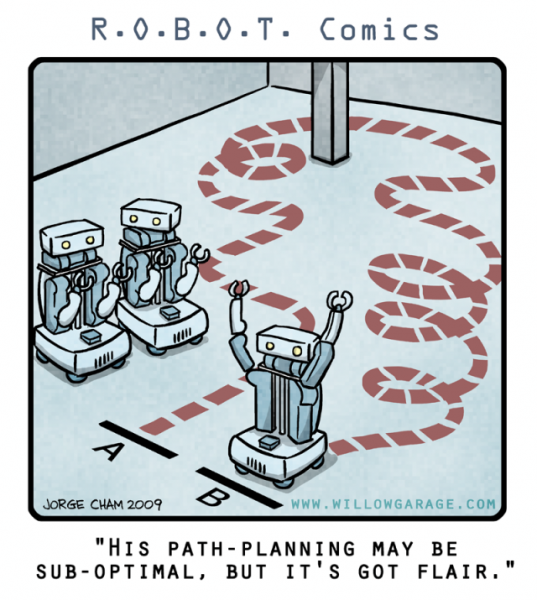
\includegraphics[width = 0.6\linewidth]
        {src/chap0-introduction/optimal-motion-planning.png}}
      \caption{A robot solves a motion planning problem to connect
        point A to point B. The solution is collision-free, but
        obviously the robot can do much better (Courtesy of Jorge
        Cham, PhD Comics).}
      \label{fig:chap0-optimal-motion-planning}
\end{figure}

\section{Contributions}

\emph{The first contribution} of this thesis is a heuristic and
efficient optimization method that takes as input a path computed for
the robot bounding box, and produces a path where a discrete set of
configurations is reoriented using an A* search algorithm. The
resulting trajectory is realistic and time-optimal. This method is
validated in various scenarios.

\emph{The second contribution} is a whole-body motion planner for
humanoid robots which computes collision-free walking trajectories,
based on exact models of both robot and environment. It is used to
solve manipulation tasks that may require walking. The first stage of
our algorithm uses a sampling-based constrained motion planner and
computes a collision-free statically balanced path for a robot which
can be fixed or sliding on the ground. The formal proof that dynamic
walking makes humanoid robots small-space controllable is then
established; this has a direct implication that this first path can
always be approximated by a dynamically balanced, collision-free
walking trajectory. This well-grounded method is implemented and the
results are validated in several environments.

In a \emph{third contribution}, a new framework for optimal motion
planning is proposed. Given a humanoid robot geometric and dynamic
model, an exact model of the environment, start and end
configurations, and a robot contact stance, we first plan a
collision-free statically balanced path that satisfies all
kinematic constraints. We convert the path to an initial trajectory
using a suitable time parametrization, and we then optimize it
to generate a locally-optimal collision-free
dynamically-balanced trajectory. This involves both finding a
new time parametrization for the trajectory, and reshaping the path in
a geometrical sense, so it is not simply a problem of optimal path
tracking. In order to ensure (self-)collision avoidance during the
optimization process, we choose to model distance constraints using
bounding capsules around the robot exact body geometries. We provide
an automatic bounding capsule generation tool; it relies on a
numerical optimization problem formulation that allows us to find the
minimum-volume capsules around bodies which are modeled by
polyhedrons. The capsules allow us then to enforce collision-avoidance
constraints between the robot, obstacles and itself.

Finally, special care was given in this thesis to generate feasible
motions that can be not only executed on digital actors, but also on
physical humanoid robots in real environments. Therefore, resulting
motions from all previously cited contributions were successfully
executed on the HRP-2 humanoid robot \cite{kane04}.

\section{Outline of This Thesis}

The thesis is organized by contribution, and related state-of-the-art
work is described when needed. Chapter \ref{chap:path-optim} describes
the path optimization method for humanoid walk planning. Chapter
\ref{chap:wholebody-planning} deals with the second contribution,
namely whole body motion planning and the associated small-space
controllability proof. Finally, the optimal motion planning framework
and the automatic bounding capsule generator are portrayed in Chapter
\ref{chap:optimal-motion-planning}.
